\chapter{Algorithms}
\label{chap:algorithms}

In the algorithms chapter we introduce four fundamental algorithms to that are often used in various combinations to model problems in parallel.~\cite{udacity}
We will be introducing map (\cref{sec:map}), reduce (\cref{sec:reduce}), scan (\cref{sec:scan}) and histogram (\cref{sec:histogram}).
Furthermore, we present the compact algorithm (\cref{sec:compact}), and radix sort (\cref{sec:radix sort}), which uses these basic algorithms to solve more complex problems.

Moreover, in the first three sections we present plots to illustrate the runtime's development while we expand the array size of the input from $2^0$ to $2^{29}$.
We performed these tests by running each array size 10 times and averaging the runtime results.
So, we ran $30 \times 10$ total runs for each test.

\section{Debugging}
\label{sec:debugging and profiling}
To debug we use two approached; \ttt{printf} for testing the logic of our application and \ttt{cuda-memcheck} to catch cuda memory errors.

The \ttt{cuda-memcheck} is a command-line tool that allows print of captured cuda-errors doing runtime.
It can be used to find issues with memory access, thread ordering, race conditions and hardware reported program errors.
It is invoked as folllows
%
\begin{quote}
  \ttt{cuda-memcheck [options] application-name [application-options]}
\end{quote}
%
As with the \ttt{nvprof} from \cref{sec:introduction to analysis of optimisation} the \ttt{cuda-memcheck} tool has a variety of flags for the option input.
In the option input \ttt{memcheck} is sat by default.
We further tested the option flag \ttt{racecheck}.
The \ttt{racecheck} allows us to detect write-after-write hazards, where two or more threads attempt to update the same memory location simultaneously.
For example, our race condition from \cref{sec:challenges with parallel programs} gave the following stacktrace\todo{outprint}.~\cite{cudamemcheck2015doc}

\section{Map}
\label{sec:map}

\Cref{lst:map par} shows the map kernel.

\begin{lstlisting}[caption={Map kernel}, label={lst:map par}]
__global__ 
void map_kernel(int *d_out, int *d_in, int SIZE) {
  int mid = threadIdx.x + blockDim.x * blockIdx.x;
  if (mid >= SIZE) return; // checking for out-of-bounds
  d_out[mid] = d_in[mid];
}
\end{lstlisting}

\Cref{lst:map seq} shows the serial code for map.

\begin{lstlisting}[caption={Serial map}, label={lst:map seq}]
void map(int *h_in, int *h_out, int SIZE) {
  for (int j = 0; j < SIZE; j++) 
    h_out[j] = h_in[j];
}
\end{lstlisting}

\section{Reduce}
\label{sec:reduce}

Another handy algorithm is the reduce algorithm.
The idea is to perform some binary operation on the collection of elements in some array, and return a single result.
This operation could for instance be a sum over all elements, where the operation would be addition.
The operation must be associative, i.e. \ttt{(a op b) op c = a op (b op c)}, for the reduce algorithm to perform correctly.
\Cref{lst:reduce seq} shows the serial reduce code.
The operation loops through all input elements and sums the result.

\begin{lstlisting}[caption={Serial reduce}, label={lst:reduce seq}]
void reduce(int *h_in, int h_out, int SIZE) {
  for (int l = 0; l < SIZE; ++l) 
    h_out += h_in[l];
}
\end{lstlisting}

The challenge with the reduce code is that we perform all operations on a single memory address.
If the serial code is naively made parallel we have a race condition.
We need to split the problem into smaller problems and perform several sweeps on the results and combine the intermediary results to get the final result.
We present an illustration in \cref{fig:reduce decomp example} to try to give an intuition of how the parallel code will run.~\cite{reduceharris}

\begin{figure}[htb]
  \centering
  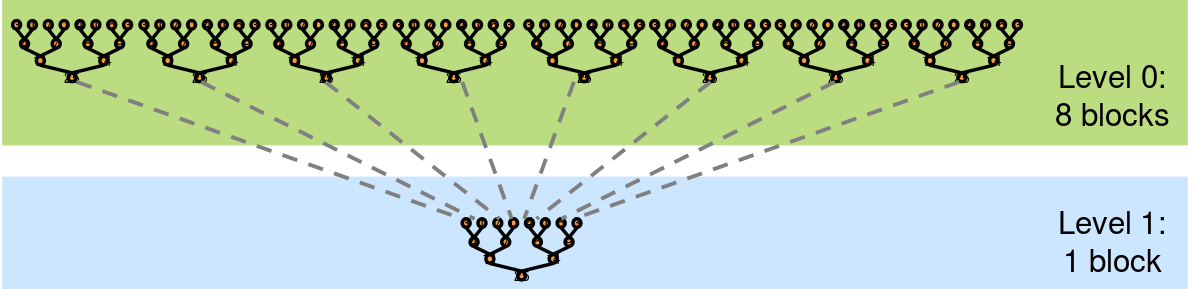
\includegraphics[width=.8\textwidth]{images/reduce_decomp_example.png}
  \caption{Reducing over multiple sweeps}
  \label{fig:reduce decomp example}
\end{figure}

The idea is that each block in the image is performed by each kernel invocation.
\Cref{lst:reduce par} shows the reduce kernel.
The needed indices are calculated, followed by the block's reduction in the loop.
Before proceeding the code makes sure that all threads have finished.
Finally, only the first thread writes the block's reduction to the output array.
The output is written to the block's index in the grid, which makes sure that each block's result is written to independent addresses.

\begin{lstlisting}[caption={Reduce kernel}, label={lst:reduce par}]
__global__
void reduce_kernel(int *d_out, int *d_in, int SIZE) {
  int mid = threadIdx.x + blockIdx.x * blockDim.x,
      tid = threadIdx.x;

  for (int s = blockDim.x / 2; s > 0; s /= 2) {
    if ((tid < s) && ((mid + s) < SIZE))
      d_in[mid] += d_in[mid + s];
    __syncthreads();
  }

  if ((tid == 0) && (mid < SIZE))
    d_out[blockIdx.x] = d_in[mid];
}
\end{lstlisting}

The intermediate results are thus transferred to the next iteration of kernel invocations.
We add a wrapper function, in \cref{lst:reduce wrapper}, that runs these kernels iteratively.
We introduce temporary arrays to hold the intermediate results, and update the grid size number of elements accordingly before invoking the kernel again.
Finally, the code performs a final invocation of the kernel with the desired final output array to combine the results.

\begin{lstlisting}[caption={The loop in the wrapper for the reduce kernel}, label={lst:reduce wrapper}]
do {
  reduce_kernel<<<grid_size, BLOCK_SIZE>>>(d_tmp_out, d_tmp_in, size);
  // Updating intermediate arrays
  size  = grid_size;
  bytes = sizeof(int) * size;
  cudaMemcpy(d_tmp_in, d_tmp_out, bytes, cudaMemcpyDeviceToDevice);
  // Updating to reflect how many blocks we now want to compute on
  grid_size = size / BLOCK_SIZE + ((size % BLOCK_SIZE)?1:0);
} while(size > BLOCK_SIZE);
// Computing remainder
reduce_kernel<<<1, size>>>(d_out, d_tmp_out, size);
\end{lstlisting}

\subsection{Using Shared Memory}
\label{sec: reduce shared memory}

A rather quick optimisation is to use shared memory instead of global memory in the kernel.
The kernel performs read and write operations in the l
If we have 1024 threads per block then we will do more than 3000 read and write operations to global memory.
However, if we read the needed memory into shared memory and perform the loop on that memory, then we will do about 1000 read and write operations.
Thus, we can achieve a theoretical 3x speed up.
The number of read and writes are presented in \cref{tab:reduce global to shared}.

\begin{table}[htb]
  \centering
  \begin{tabular}{c r | r r r r r}
    \toprule
    \multirow{2}*{global memory} & read  & 1024 & 512 & 256 & $\cdots$ & 1 \\
                                 & write &  512 & 256 & 128 & $\cdots$ & 1 \\
    \midrule
    \multirow{2}*{shared memory} & read  & 1024 & & &  &  \\
                                 & write &    1 & & &  &  \\
    \bottomrule
  \end{tabular}
  \caption{Global vs. Shared memory read and writes}
  \label{tab:reduce global to shared}
\end{table}

We present the revised reduce kernel with shared memory in \cref{lst:reduce par shared}.
We add the \ttt{sdata} array to contain the shared memory, and each thread copies the global data to that shared memory.


\begin{lstlisting}[caption={Reduce kernel using shared memory}, label={lst:reduce par shared}]
__global__
void reduce_kernel(int *d_out, int *d_in, int SIZE) {
  int mid = threadIdx.x + blockIdx.x * blockDim.x,
      tid = threadIdx.x;
  if (mid >= SIZE) return;

  extern __shared__ int sdata[]; // allocate shared memory
  sdata[tid] = d_in[mid];        // each thread loads global to shared memory
  __syncthreads();               // make sure all threads are done

  for (int s = blockDim.x / 2; s > 0; s /= 2) {
    if ((tid < s) && ((mid + s) < SIZE))
      sdata[tid] += sdata[tid + s]; // perform operations on shared memory
    __syncthreads();
  }

  if ((tid == 0) && (mid < SIZE))
    d_out[blockIdx.x] = sdata[0];   // copy shared back to global memory
}
\end{lstlisting}

\begin{lstlisting}[caption={Updated call to reduce kernel after use of shared memory}, label={lst:reduce invocation with smem}]
const unsigned int SMEM = BLOCK_SIZE * sizeof(int);
reduce_kernel<<<grid_size, BLOCK_SIZE, SMEM>>>(d_tmp_out, d_tmp_in, size);
\end{lstlisting}

Furthermore, we must update the kernel call to include the amount of shared memory to be allocated.
This is illustrated in \cref{lst:reduce invocation with smem}, where the third argument in the triple chevrons is the amount of shared memory to allocate

We present a plot in \cref{fig:reduce plot} illustrating the development of the run time for the reduce algorithms presented.
The GPGPU gets an advantage when the array size to sum is large.
This is most likely due to that fact that the CPU is much faster than the GPGPU.
The GPGPU beats the CPU when it has enough work to spread out to its threads.

\begin{figure}[htb]
  \centering
  \section{Reduce}
\label{sec:reduce}

Another handy algorithm is the reduce algorithm.
The idea is to perform some binary operation on the collection of elements in some array, and return a single result.
This operation could for instance be a sum over all elements, where the operation would be addition.
The operation must be associative, i.e. \ttt{(a op b) op c = a op (b op c)}, for the reduce algorithm to perform correctly.
\Cref{lst:reduce seq} shows the serial reduce code.
The operation loops through all input elements and sums the result.

\begin{lstlisting}[caption={Serial reduce}, label={lst:reduce seq}]
void reduce(int *h_in, int h_out, int SIZE) {
  for (int l = 0; l < SIZE; ++l) 
    h_out += h_in[l];
}
\end{lstlisting}

The challenge with the reduce code is that we perform all operations on a single memory address.
If the serial code is naively made parallel we have a race condition.
We need to split the problem into smaller problems and perform several sweeps on the results and combine the intermediary results to get the final result.
We present an illustration in \cref{fig:reduce decomp example} to try to give an intuition of how the parallel code will run.~\cite{reduceharris}

\begin{figure}[htb]
  \centering
  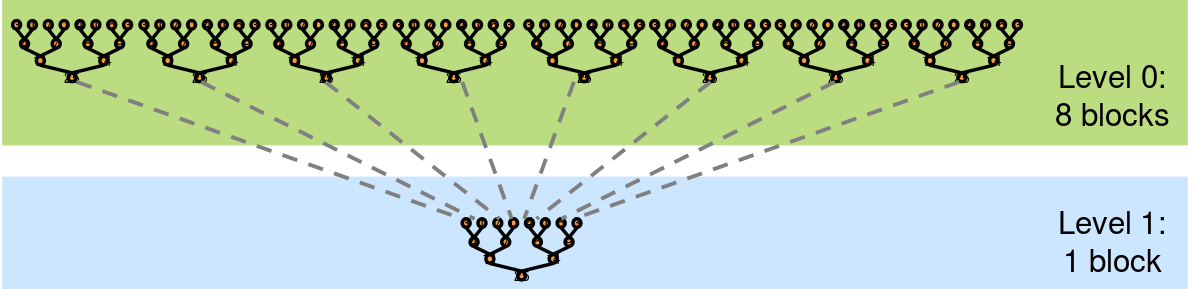
\includegraphics[width=.8\textwidth]{images/reduce_decomp_example.png}
  \caption{Reducing over multiple sweeps}
  \label{fig:reduce decomp example}
\end{figure}

The idea is that each block in the image is performed by each kernel invocation.
\Cref{lst:reduce par} shows the reduce kernel.
The needed indices are calculated, followed by the block's reduction in the loop.
Before proceeding the code makes sure that all threads have finished.
Finally, only the first thread writes the block's reduction to the output array.
The output is written to the block's index in the grid, which makes sure that each block's result is written to independent addresses.

\begin{lstlisting}[caption={Reduce kernel}, label={lst:reduce par}]
__global__
void reduce_kernel(int *d_out, int *d_in, int SIZE) {
  int mid = threadIdx.x + blockIdx.x * blockDim.x,
      tid = threadIdx.x;

  for (int s = blockDim.x / 2; s > 0; s /= 2) {
    if ((tid < s) && ((mid + s) < SIZE))
      d_in[mid] += d_in[mid + s];
    __syncthreads();
  }

  if ((tid == 0) && (mid < SIZE))
    d_out[blockIdx.x] = d_in[mid];
}
\end{lstlisting}

The intermediate results are thus transferred to the next iteration of kernel invocations.
We add a wrapper function, in \cref{lst:reduce wrapper}, that runs these kernels iteratively.
We introduce temporary arrays to hold the intermediate results, and update the grid size number of elements accordingly before invoking the kernel again.
Finally, the code performs a final invocation of the kernel with the desired final output array to combine the results.

\begin{lstlisting}[caption={The loop in the wrapper for the reduce kernel}, label={lst:reduce wrapper}]
do {
  reduce_kernel<<<grid_size, BLOCK_SIZE>>>(d_tmp_out, d_tmp_in, size);
  // Updating intermediate arrays
  size  = grid_size;
  bytes = sizeof(int) * size;
  cudaMemcpy(d_tmp_in, d_tmp_out, bytes, cudaMemcpyDeviceToDevice);
  // Updating to reflect how many blocks we now want to compute on
  grid_size = size / BLOCK_SIZE + ((size % BLOCK_SIZE)?1:0);
} while(size > BLOCK_SIZE);
// Computing remainder
reduce_kernel<<<1, size>>>(d_out, d_tmp_out, size);
\end{lstlisting}

\subsection{Using Shared Memory}
\label{sec: reduce shared memory}

A rather quick optimisation is to use shared memory instead of global memory in the kernel.
The kernel performs read and write operations in the l
If we have 1024 threads per block then we will do more than 3000 read and write operations to global memory.
However, if we read the needed memory into shared memory and perform the loop on that memory, then we will do about 1000 read and write operations.
Thus, we can achieve a theoretical 3x speed up.
The number of read and writes are presented in \cref{tab:reduce global to shared}.

\begin{table}[htb]
  \centering
  \begin{tabular}{c r | r r r r r}
    \toprule
    \multirow{2}*{global memory} & read  & 1024 & 512 & 256 & $\cdots$ & 1 \\
                                 & write &  512 & 256 & 128 & $\cdots$ & 1 \\
    \midrule
    \multirow{2}*{shared memory} & read  & 1024 & & &  &  \\
                                 & write &    1 & & &  &  \\
    \bottomrule
  \end{tabular}
  \caption{Global vs. Shared memory read and writes}
  \label{tab:reduce global to shared}
\end{table}

We present the revised reduce kernel with shared memory in \cref{lst:reduce par shared}.
We add the \ttt{sdata} array to contain the shared memory, and each thread copies the global data to that shared memory.


\begin{lstlisting}[caption={Reduce kernel using shared memory}, label={lst:reduce par shared}]
__global__
void reduce_kernel(int *d_out, int *d_in, int SIZE) {
  int mid = threadIdx.x + blockIdx.x * blockDim.x,
      tid = threadIdx.x;
  if (mid >= SIZE) return;

  extern __shared__ int sdata[]; // allocate shared memory
  sdata[tid] = d_in[mid];        // each thread loads global to shared memory
  __syncthreads();               // make sure all threads are done

  for (int s = blockDim.x / 2; s > 0; s /= 2) {
    if ((tid < s) && ((mid + s) < SIZE))
      sdata[tid] += sdata[tid + s]; // perform operations on shared memory
    __syncthreads();
  }

  if ((tid == 0) && (mid < SIZE))
    d_out[blockIdx.x] = sdata[0];   // copy shared back to global memory
}
\end{lstlisting}

\begin{lstlisting}[caption={Updated call to reduce kernel after use of shared memory}, label={lst:reduce invocation with smem}]
const unsigned int SMEM = BLOCK_SIZE * sizeof(int);
reduce_kernel<<<grid_size, BLOCK_SIZE, SMEM>>>(d_tmp_out, d_tmp_in, size);
\end{lstlisting}

Furthermore, we must update the kernel call to include the amount of shared memory to be allocated.
This is illustrated in \cref{lst:reduce invocation with smem}, where the third argument in the triple chevrons is the amount of shared memory to allocate

We present a plot in \cref{fig:reduce plot} illustrating the development of the run time for the reduce algorithms presented.
The GPGPU gets an advantage when the array size to sum is large.
This is most likely due to that fact that the CPU is much faster than the GPGPU.
The GPGPU beats the CPU when it has enough work to spread out to its threads.

\begin{figure}[htb]
  \centering
  \section{Reduce}
\label{sec:reduce}

Another handy algorithm is the reduce algorithm.
The idea is to perform some binary operation on the collection of elements in some array, and return a single result.
This operation could for instance be a sum over all elements, where the operation would be addition.
The operation must be associative, i.e. \ttt{(a op b) op c = a op (b op c)}, for the reduce algorithm to perform correctly.
\Cref{lst:reduce seq} shows the serial reduce code.
The operation loops through all input elements and sums the result.

\begin{lstlisting}[caption={Serial reduce}, label={lst:reduce seq}]
void reduce(int *h_in, int h_out, int SIZE) {
  for (int l = 0; l < SIZE; ++l) 
    h_out += h_in[l];
}
\end{lstlisting}

The challenge with the reduce code is that we perform all operations on a single memory address.
If the serial code is naively made parallel we have a race condition.
We need to split the problem into smaller problems and perform several sweeps on the results and combine the intermediary results to get the final result.
We present an illustration in \cref{fig:reduce decomp example} to try to give an intuition of how the parallel code will run.~\cite{reduceharris}

\begin{figure}[htb]
  \centering
  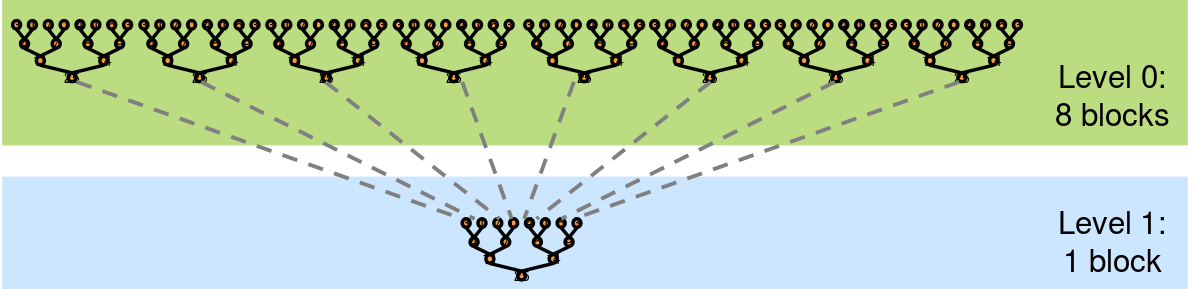
\includegraphics[width=.8\textwidth]{images/reduce_decomp_example.png}
  \caption{Reducing over multiple sweeps}
  \label{fig:reduce decomp example}
\end{figure}

The idea is that each block in the image is performed by each kernel invocation.
\Cref{lst:reduce par} shows the reduce kernel.
The needed indices are calculated, followed by the block's reduction in the loop.
Before proceeding the code makes sure that all threads have finished.
Finally, only the first thread writes the block's reduction to the output array.
The output is written to the block's index in the grid, which makes sure that each block's result is written to independent addresses.

\begin{lstlisting}[caption={Reduce kernel}, label={lst:reduce par}]
__global__
void reduce_kernel(int *d_out, int *d_in, int SIZE) {
  int mid = threadIdx.x + blockIdx.x * blockDim.x,
      tid = threadIdx.x;

  for (int s = blockDim.x / 2; s > 0; s /= 2) {
    if ((tid < s) && ((mid + s) < SIZE))
      d_in[mid] += d_in[mid + s];
    __syncthreads();
  }

  if ((tid == 0) && (mid < SIZE))
    d_out[blockIdx.x] = d_in[mid];
}
\end{lstlisting}

The intermediate results are thus transferred to the next iteration of kernel invocations.
We add a wrapper function, in \cref{lst:reduce wrapper}, that runs these kernels iteratively.
We introduce temporary arrays to hold the intermediate results, and update the grid size number of elements accordingly before invoking the kernel again.
Finally, the code performs a final invocation of the kernel with the desired final output array to combine the results.

\begin{lstlisting}[caption={The loop in the wrapper for the reduce kernel}, label={lst:reduce wrapper}]
do {
  reduce_kernel<<<grid_size, BLOCK_SIZE>>>(d_tmp_out, d_tmp_in, size);
  // Updating intermediate arrays
  size  = grid_size;
  bytes = sizeof(int) * size;
  cudaMemcpy(d_tmp_in, d_tmp_out, bytes, cudaMemcpyDeviceToDevice);
  // Updating to reflect how many blocks we now want to compute on
  grid_size = size / BLOCK_SIZE + ((size % BLOCK_SIZE)?1:0);
} while(size > BLOCK_SIZE);
// Computing remainder
reduce_kernel<<<1, size>>>(d_out, d_tmp_out, size);
\end{lstlisting}

\subsection{Using Shared Memory}
\label{sec: reduce shared memory}

A rather quick optimisation is to use shared memory instead of global memory in the kernel.
The kernel performs read and write operations in the l
If we have 1024 threads per block then we will do more than 3000 read and write operations to global memory.
However, if we read the needed memory into shared memory and perform the loop on that memory, then we will do about 1000 read and write operations.
Thus, we can achieve a theoretical 3x speed up.
The number of read and writes are presented in \cref{tab:reduce global to shared}.

\begin{table}[htb]
  \centering
  \begin{tabular}{c r | r r r r r}
    \toprule
    \multirow{2}*{global memory} & read  & 1024 & 512 & 256 & $\cdots$ & 1 \\
                                 & write &  512 & 256 & 128 & $\cdots$ & 1 \\
    \midrule
    \multirow{2}*{shared memory} & read  & 1024 & & &  &  \\
                                 & write &    1 & & &  &  \\
    \bottomrule
  \end{tabular}
  \caption{Global vs. Shared memory read and writes}
  \label{tab:reduce global to shared}
\end{table}

We present the revised reduce kernel with shared memory in \cref{lst:reduce par shared}.
We add the \ttt{sdata} array to contain the shared memory, and each thread copies the global data to that shared memory.


\begin{lstlisting}[caption={Reduce kernel using shared memory}, label={lst:reduce par shared}]
__global__
void reduce_kernel(int *d_out, int *d_in, int SIZE) {
  int mid = threadIdx.x + blockIdx.x * blockDim.x,
      tid = threadIdx.x;
  if (mid >= SIZE) return;

  extern __shared__ int sdata[]; // allocate shared memory
  sdata[tid] = d_in[mid];        // each thread loads global to shared memory
  __syncthreads();               // make sure all threads are done

  for (int s = blockDim.x / 2; s > 0; s /= 2) {
    if ((tid < s) && ((mid + s) < SIZE))
      sdata[tid] += sdata[tid + s]; // perform operations on shared memory
    __syncthreads();
  }

  if ((tid == 0) && (mid < SIZE))
    d_out[blockIdx.x] = sdata[0];   // copy shared back to global memory
}
\end{lstlisting}

\begin{lstlisting}[caption={Updated call to reduce kernel after use of shared memory}, label={lst:reduce invocation with smem}]
const unsigned int SMEM = BLOCK_SIZE * sizeof(int);
reduce_kernel<<<grid_size, BLOCK_SIZE, SMEM>>>(d_tmp_out, d_tmp_in, size);
\end{lstlisting}

Furthermore, we must update the kernel call to include the amount of shared memory to be allocated.
This is illustrated in \cref{lst:reduce invocation with smem}, where the third argument in the triple chevrons is the amount of shared memory to allocate

We present a plot in \cref{fig:reduce plot} illustrating the development of the run time for the reduce algorithms presented.
The GPGPU gets an advantage when the array size to sum is large.
This is most likely due to that fact that the CPU is much faster than the GPGPU.
The GPGPU beats the CPU when it has enough work to spread out to its threads.

\begin{figure}[htb]
  \centering
  \input{graphics/plots/reduce}
  \caption{Runtime development of three reduce algorithms}
  \label{fig:reduce plot}
\end{figure}

We mentioned that the shared memory version of the reduce would theoretically get approximately a 3x speed-up compared to the regular version.
This is not the case as illustrated in the plot.
This is due to the fact that we do not utilize the full potential of the local memory of the device.
If we were to get closer to the theoretical speed-up we would have to do more optimisations.

  \caption{Runtime development of three reduce algorithms}
  \label{fig:reduce plot}
\end{figure}

We mentioned that the shared memory version of the reduce would theoretically get approximately a 3x speed-up compared to the regular version.
This is not the case as illustrated in the plot.
This is due to the fact that we do not utilize the full potential of the local memory of the device.
If we were to get closer to the theoretical speed-up we would have to do more optimisations.

  \caption{Runtime development of three reduce algorithms}
  \label{fig:reduce plot}
\end{figure}

We mentioned that the shared memory version of the reduce would theoretically get approximately a 3x speed-up compared to the regular version.
This is not the case as illustrated in the plot.
This is due to the fact that we do not utilize the full potential of the local memory of the device.
If we were to get closer to the theoretical speed-up we would have to do more optimisations.

\begin{tikzpicture}
  \begin{axis}[
    ymajorgrids,
    xmajorgrids,
    ylabel={Time (ms)},
    xlabel={Array size},
    xmode=log,
    log basis x={2},
    legend style={
      at={(0.05,0.95)},
      anchor=north west,
      column sep=1ex
     },
     no markers,
     very thick 
   ]

    \addplot table [x=x, y=parallel] {data/scan.csv};
    \addlegendentry{parallel};
    \addplot+[dashed] table [x=x, y=sequential] {data/scan.csv};
    \addlegendentry{sequential};
  \end{axis}
\end{tikzpicture}

\begin{tikzpicture}
  \begin{axis}[
    ymajorgrids,
    xmajorgrids,
    ylabel={Time (ms)},
    xlabel={Memory size ($2^x$)},
    xmode=log,
    log basis x={2},
    legend style={
      at={(0.05,0.95)},
      anchor=north west,
      column sep=1ex
     },
     no markers,
     very thick 
   ]

    \addplot table [x=x, y=parallel] {data/histogram.csv};
    \addlegendentry{parallel};
    \addplot table [x=x, y=sequential] {data/histogram.csv};
    \addlegendentry{sequential};
  \end{axis}
\end{tikzpicture}

\section{Compact}
\label{sec:compact}

This section presents the algorithm commonly known as compact (also known as filter).
The idea is to take some input and only return the items that obey some predicate, e.g. whether or not the least significant bit (LSB) is 0.
The algorithm can be divided into three steps
%
\begin{enumerate}
  \item Calculate predicate array
  \item Calculate scatter addresses from predicate array
  \item Map desired items to output, given the scatter addresses
\end{enumerate}
%
\Cref{lst:predicate} briefly presents a simple computation whether or not the LSB is 0, and saves the result to the \ttt{predicate} array.

\begin{lstlisting}[numbers=none, caption={LSB equal to 0 -- save items' result to predicate array.}, label={lst:predicate}]
predicate[idx] = (int)((input[idx] & 1) == 0);
\end{lstlisting}

The next step is to compute the addresses whereto the given items from the input array must be moved to.
This can be computed with an exclusive sum scan over the \ttt{predicate} array.
\Cref{tab:excl sum scan} presents a simple example, where the top row presents the input indices, then the items in each index, the predicate for that item, and the scatter address based on the predicates, respectively.

\begin{table}[htb]
  \centering
  \begin{tabular}{r | c c c c c c}
    \toprule
    \tbf{idx}             & 0 & 1 & 2 & 3 & 4 & 5 \\
    \midrule
    \tbf{items}           & 4 & 5 & 6 & 7 & 8 & 9 \\
    \tbf{predicate}       & 1 & 0 & 1 & 0 & 1 & 0 \\
    \tbf{scatter address} & 0 & 1 & 1 & 2 & 2 & 2 \\
    \bottomrule
  \end{tabular}
  \caption{Predicate and scatter address output given the input}
  \label{tab:excl sum scan}
\end{table}

From the scatter addresses it is now possible to map the values where the predicate is 1 to a new output array.
The contents of that array is thus the values where the LSB is 0.
This array will be of length 3, because the reduction of the predicate array yields the value 3.
The array will be \ttt{[4, 6, 8]}.



\section{Radix Sort}
\label{sec:radix sort}

This this section will present a parrallized algorithm of the radix sort benchmarked with a serial sort implementation from the C++ library.
The implementation of the Radix Sort algorithm can be found in \cref{ap:radix sort}.

Radix Sort is a bit-wise comparison algorithm that iteratively, in the length of the bits of the integer, looks at the LSB and sorts the values accordingly.\cite{udacity}

In order to parralelize the sorting of the LSB in the radix sort we used the compact(\cref{sec:compact}).  
Thus, the radix sort is performed with multiple compact operations, because we move elements according to some predicate.
We aim to outline a single iteration of radix sort in this section.

% iteratively do for each bit

\paragraph{Compute Predicates}
The first step is to find the elements that obey the predicate.
For radix sort we look at the LSB of every bit of the integers.
The predicate is as presented in \cref{lst:predicate radix}.

\begin{lstlisting}[caption={predicate to calculate}, label={lst:predicate radix}]
d_predicate[mid] = (int)(((d_val_src[mid] & (1 << i)) >> i) == 0)
\end{lstlisting}

The \ttt{d\_predicate} will contain 0s and 1s.
If the LSB is 0, it will contain a 1 for that element.
The elements in \ttt{d\_val\_src} are traversed and labelled accordingly.

For each iteration of the outer loop, we count the \ttt{i} variable up.
This way we can left shift the integer 1 by \ttt{i} positions to move to the next LSB in the row.
When perform the bitwise-and, and shift it back to see if it is equal to 0.

Furthermore, we save a new predicate array, \ttt{d\_predicate\_toggle}, where we save the toggled version of the original \ttt{d\_predicate}.
This array gives us the elements that did not obey the predicate.
We do this, because we must maintain the order of the elements in the output array.

\subsection*{Compute Scatter Addresses}

To be able to move the elements to their new positions according to the predicate, we can perform an exclusive sum scan of the predicate array.
This gives the addresses to which the elements must be scattered.
We performed an exclusive sum scan by first invoking a Hillis and Steele inclusive sum scan and then shifting the resulting array to obtain an exclusive sum scan.

For the toggled predicate array we must include an offset that is equal to the amount of elements, that did obey the initial predicate.
Thus, we must add an offset to the scatter addresses computed from the toggled predicate array.
We do this by performing a reduce operation on the original predicate array, which gives us the amount of elements that had LSB to 0.
We then do a mapping operation to add the offset to each element of the scatter address array.

The elements should then be scattered to the new addresses according to the LSB.
This is briefly illustrated in \cref{fig:radix sort example}.
This method should then be continued for each bit.
We continue to the next bit by incrementing the variable \ttt{i}, and perform the bitwise-and as illustrated in \cref{lst:predicate radix}.

\begin{figure}[htb]
  \centering
  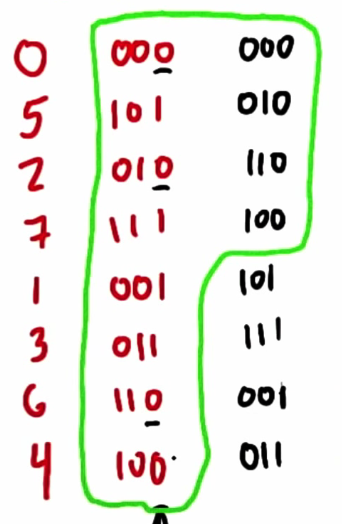
\includegraphics[height=4cm]{images/radix-sort-example.png}
  \caption{Example of how each digit is moved according to LSB}
  \label{fig:radix sort example}
\end{figure}


%\subsection*{Iterating through each Bit}
%
%\begin{lstlisting}
%for ( unsigned int i = 0; i < (BITS_PER_BYTE * sizeof( unsigned int)); i++) {
%  // predicate is that LSB is 0
%  predicate_kernel<<<GRID_SIZE, BLOCK_SIZE>>>(d_predicate, d_val_src, NUM_ELEMS, i);
%  // calculate scatter addresses from predicates
%  exclusive_sum_scan(d_sum_scan_0, d_predicate, d_predicate_tmp, d_sum_scan, ARRAY_BYTES, NUM_ELEMS, GRID_SIZE, BLOCK_SIZE);
%  // copy contents of predicate , so we do not change its content
%  checkCudaErrors(cudaMemcpy(d_predicate_tmp, d_predicate, ARRAY_BYTES, cudaMemcpyDeviceToDevice));
%  // calculate how many elements had predicate equal to 1
%  reduce_wrapper(d_reduce, d_predicate_tmp, NUM_ELEMS, BLOCK_SIZE);
%  // toggle predicate values , so we can compute scatter addresses for toggled predicates
%  toggle_predicate_kernel<<<GRID_SIZE, BLOCK_SIZE>>>(d_predicate_toggle ,d_predicate, NUM_ELEMS);
%  // so we now have addresses for elements where LSB is equal to 1
%  exclusive_sum_scan(d_sum_scan_1, d_predicate_toggle, d_predicate_tmp, d_sum_scan, ARRAY_BYTES, NUM_ELEMS, GRID_SIZE, BLOCK_SIZE);
%  // shift scatter addresses according to amount of elements that had LSB equal to 0
%  add_splitter_map_kernel<<<GRID_SIZE, BLOCK_SIZE>>>(d_sum_scan_1, d_reduce, NUM_ELEMS);
%  // move elements accordingly
%  map_kernel<<<GRID_SIZE, BLOCK_SIZE>>>(d_map, d_val_src, d_predicate, d_sum_scan_0, d_sum_scan_1, NUM_ELEMS);
%  // swap pointers , instead of moving elements
%  std::swap(d_val_src, d_map);
%}
%\end{lstlisting}

